\section{Passive buzzer}
\begin{figure}[H]
    \centering
    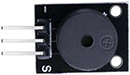
\includegraphics[angle=0, keepaspectratio=true, scale=1, width=200px, height=200px]{images/buzzer2.jpg}
    %\caption{Caption}
\end{figure}
\subsection*{Description}
A passive buzzer has no internal oscillator and requires a PWM signal to operate. By varying the duty cycle and frequency of the PWM signal applied to the passive buzzer the tone and pitch can be varied.
\subsection*{Pin mapping}
This pin mapping corresponds to the pins from left to right with the module pins facing towards you.
\begin{table}[H]
    \centering
    \begin{tabular}{|c|c|c|c|c|}
    \hline
    Index &Label &Type &Name &Description\\ \hline
    0 &- &Ground &GND &\\ \hline
    1 & &Source voltage &$V+$ &Module source voltage ($5V$)\\ \hline
    2 &S &Analog input &A0 &DC or PWM signal to control buzzer\\ \hline
    \end{tabular}
    %\caption{Caption}
    %\label{tab:my_label}
\end{table}
\subsection*{Operation}
Setting the analog input pin A0 of the buzzer module to high will turn on produce no tone. By applying a PWM signal to A0 the tone and pitch of the buzzer can be varied.
\subsection*{Code}
Refer to listing \ref{python_buzzer}.
%\lstinputlisting[caption=test]{laser.py}